\section{Paradigm shift}

The usual client-server paradigm demands to have two separate entities:
\begin{itemize}
    \item Client: it's software runs on end-hosts, it has an on/off behavior.
    It consumes the service offered by the server by issuing requests to it.
    Clients usually do not communicate directly among them but always via the server.
    Clients need to know the server IP in order to connect and interact with it.

    \item Server: the server software runs on a dedicated hosts and it is necessary that it is always on.
    It provides the service which is then consumed by the clients by receiving and responding to requests.
    It needs to have a fixed IP or a DNS name in order to be easily found.
\end{itemize}

In a peer-to-peer system instead each host is an end-hosts.
Each single node has an on/off behavior and it is needed to handle churn (continuous change of nodes in the network).
There is the problem of joining the network because it is not sure that you know the address of a node currently in the network.
Once joined the network there is the problem of discovering other peers, locating resources on the server and providing them.

There is the needs to define communication rules in order to prevent free riding and incentivate participation and reciprocation.

In a p2p network servers are still used in order to bootstrap the network, but once the network is up and running they can be turned off cause those aren't needed for resource sharing.

\subsection{A general definition}
A peer to peer system is a set of \emph{autonomous entities} able to \emph{auto-organize} and sharing a set of distributed resources in a computer network.
The system exploits such resources to give a service in a \emph{complete or partial decentralized way}.

Some example of shared resources could be:
\begin{itemize}
    \item ledger (like on the blockchain);
    \item read/write storage space (like on a distributed file system);
    \item computing power;
    \item bandwidth.
\end{itemize}

\subsection{Another definition}
A p2p system is a distributed system defined by a set of nodes interconnected albe to \emph{auto-organize} and to build different topologies with the goal of \emph{sharing resources} like CPU cycles, memory, bandwidth.
The system is able to adapt to a \emph{continuous churn} of the nodes maintaining connectivity and reasonable performances without a centralized entity (like a server).

\subsection{Resource sharing}
P2P is relative to give and receive from a community: each peer should share a set of resources and obtain in return another set of resources or services, behaving symmetrically (\emph{servent}).
Some famous examples are related to file sharing like music, film, and other (Napster, Gnutella, Bittorret, etc).

But in some network a peer offer resources for free, maybe to participate to a project like \emph{SETI@home} in which people give computational power in order to analyze data looking for extra-terrestrial life.

In some other networks instead peers are rewarded for contributing to the management of the network like in blockchains, in which miners are rewarded with coins.

The main idea though is that shared resources are at the border of the internet and are directly shared by the peers, without special purpose nodes.

\section{Killer applications}

\subsection{File sharing (put example here)}

\subsection{Blockchain}
Let's give some definition before discussing it properly:
\begin{itemize}
    \item a shared database in multiple copies on computers throughout the world, maintained without the need for a central authority (like a bank, a company, a state, etc);
    \item replicated and consistent, immutable, append-only data storage system resistant to tampering;
    \item a write-only, decentralized, state machine that is maintained by untrusted actors, secured by economic incentive. On that machine data cannot be deleted, the machine cannot be shut down or censored and it supports defined operations agreed upon by participants.
    Participants may not know each other but the best interest is to play by the rules.
\end{itemize}

The blockchain abstraction is built on:
\begin{itemize}
    \item digital signature, to provide authentication;
    \item cryptographic hash functions, to provide tamper-resistant immutability;
    \item replication to provide availability;
    \item distributed consensus among mutually trusting or distrusting replica, to provide integrity and decentralized control.
\end{itemize}

\subsubsection{Blockchain taxonomy}
Blockchains are classified based on type of access and on permissions associated:
\begin{itemize}
    \item Public and permissionless: ledges are public and everyone can be involved in the blockchain, those can suffers from scalability and privacy. Some examples are Bitcoin and Ethereum;

    \item Public and permissioned: everyone can partecipate but there is some kind of access control layer. An eample is ripple;

    \item Private and permissionless: not everyone can enroll but then there is no control layer;

    \item Private and permissioned.
\end{itemize}

\subsubsection{When to use a Blokchain}
\begin{figure}[H]
    \centering
    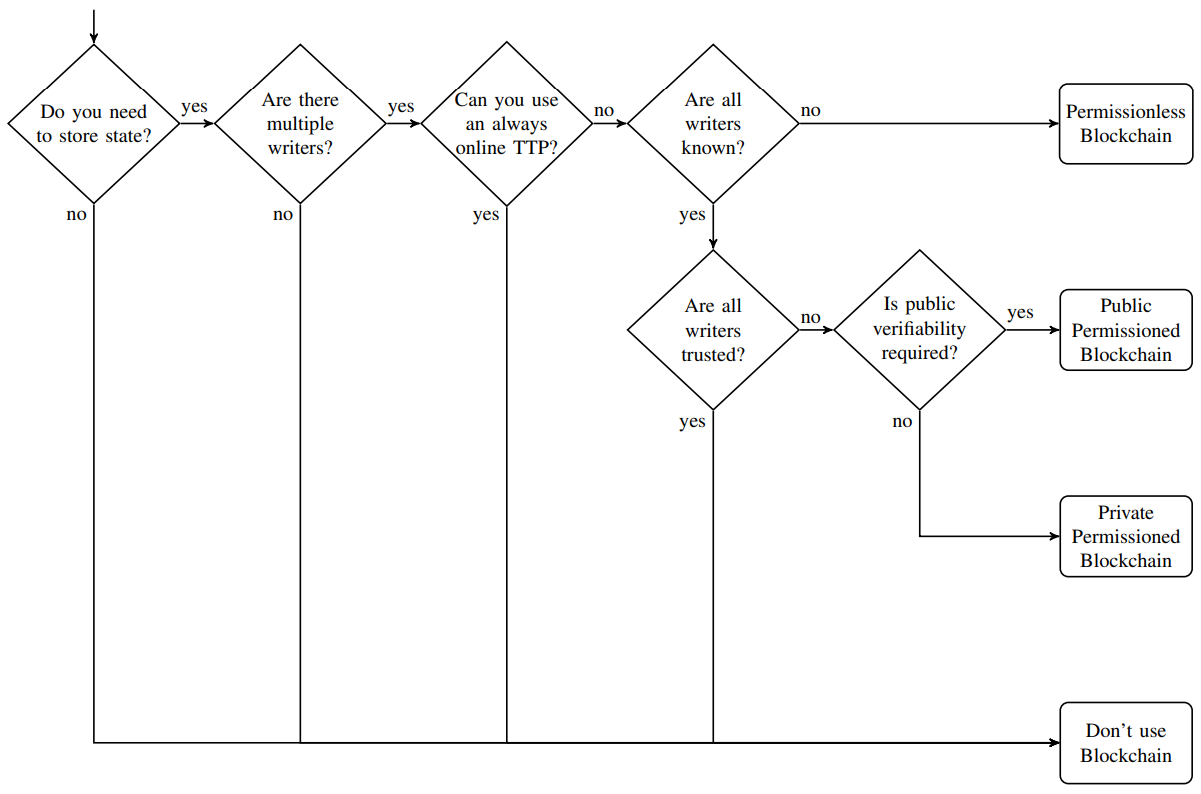
\includegraphics[width=330px]{images/1_Introduction/01.png}
    \caption{Do you need a blockchain?}
    \label{fig:enter-label}
\end{figure}

Basically the target applications for blockchains are the one that:
\begin{itemize}
    \item require shared common, append-only database with limited capacity;
    \item have multiple participants with varying degrees of trust amongst them;
    \item must run in a distributed manner;
    \item require a complex settlement process with a trusted third party;
    \item needs integrity, authentication and non-repudiation;
    \item are governed by a precise rules that do not change and re simple to encode;
    \item require transparency.
\end{itemize}

\subsubsection{Blockchain trilemma}
The biggest scientific challenge around blockchain is known as trilemma: is it possible to have a blockchain which both implement scalability, security and decentralization?
At the moment the answer is no, if you have high security and decentralization you must lack of scalability and so on.



